% Options for packages loaded elsewhere
\PassOptionsToPackage{unicode}{hyperref}
\PassOptionsToPackage{hyphens}{url}
\PassOptionsToPackage{dvipsnames,svgnames,x11names}{xcolor}
%
\documentclass[
  11pt,
]{article}
\usepackage{amsmath,amssymb}
\usepackage{iftex}
\ifPDFTeX
  \usepackage[T1]{fontenc}
  \usepackage[utf8]{inputenc}
  \usepackage{textcomp} % provide euro and other symbols
\else % if luatex or xetex
  \usepackage{unicode-math} % this also loads fontspec
  \defaultfontfeatures{Scale=MatchLowercase}
  \defaultfontfeatures[\rmfamily]{Ligatures=TeX,Scale=1}
\fi
\usepackage{lmodern}
\ifPDFTeX\else
  % xetex/luatex font selection
\fi
% Use upquote if available, for straight quotes in verbatim environments
\IfFileExists{upquote.sty}{\usepackage{upquote}}{}
\IfFileExists{microtype.sty}{% use microtype if available
  \usepackage[]{microtype}
  \UseMicrotypeSet[protrusion]{basicmath} % disable protrusion for tt fonts
}{}
\makeatletter
\@ifundefined{KOMAClassName}{% if non-KOMA class
  \IfFileExists{parskip.sty}{%
    \usepackage{parskip}
  }{% else
    \setlength{\parindent}{0pt}
    \setlength{\parskip}{6pt plus 2pt minus 1pt}}
}{% if KOMA class
  \KOMAoptions{parskip=half}}
\makeatother
\usepackage{xcolor}
\usepackage[margin=2.5cm]{geometry}
\usepackage{longtable,booktabs,array}
\usepackage{calc} % for calculating minipage widths
% Correct order of tables after \paragraph or \subparagraph
\usepackage{etoolbox}
\makeatletter
\patchcmd\longtable{\par}{\if@noskipsec\mbox{}\fi\par}{}{}
\makeatother
% Allow footnotes in longtable head/foot
\IfFileExists{footnotehyper.sty}{\usepackage{footnotehyper}}{\usepackage{footnote}}
\makesavenoteenv{longtable}
\usepackage{graphicx}
\makeatletter
\def\maxwidth{\ifdim\Gin@nat@width>\linewidth\linewidth\else\Gin@nat@width\fi}
\def\maxheight{\ifdim\Gin@nat@height>\textheight\textheight\else\Gin@nat@height\fi}
\makeatother
% Scale images if necessary, so that they will not overflow the page
% margins by default, and it is still possible to overwrite the defaults
% using explicit options in \includegraphics[width, height, ...]{}
\setkeys{Gin}{width=\maxwidth,height=\maxheight,keepaspectratio}
% Set default figure placement to htbp
\makeatletter
\def\fps@figure{htbp}
\makeatother
\setlength{\emergencystretch}{3em} % prevent overfull lines
\providecommand{\tightlist}{%
  \setlength{\itemsep}{0pt}\setlength{\parskip}{0pt}}
\setcounter{secnumdepth}{-\maxdimen} % remove section numbering
\ifLuaTeX
\usepackage[bidi=basic]{babel}
\else
\usepackage[bidi=default]{babel}
\fi
\babelprovide[main,import]{english}
% get rid of language-specific shorthands (see #6817):
\let\LanguageShortHands\languageshorthands
\def\languageshorthands#1{}
\ifLuaTeX
  \usepackage{selnolig}  % disable illegal ligatures
\fi
\IfFileExists{bookmark.sty}{\usepackage{bookmark}}{\usepackage{hyperref}}
\IfFileExists{xurl.sty}{\usepackage{xurl}}{} % add URL line breaks if available
\urlstyle{same}
\hypersetup{
  pdftitle={US Tariffs of 2026 and German Districts: Regional Exposure of Manufacturing},
  pdfauthor={Wolf-Fabian Hungerland},
  pdflang={en},
  colorlinks=true,
  linkcolor={black},
  filecolor={Maroon},
  citecolor={Blue},
  urlcolor={blue},
  pdfcreator={LaTeX via pandoc}}

\title{US Tariffs of 2026 and German Districts: Regional Exposure of
Manufacturing}
\usepackage{etoolbox}
\makeatletter
\providecommand{\subtitle}[1]{% add subtitle to \maketitle
  \apptocmd{\@title}{\par {\large #1 \par}}{}{}
}
\makeatother
\subtitle{District exposure, local business tax and regional aid}
\author{Wolf-Fabian Hungerland}
\date{Draft, 12 November 2026}

\begin{document}
\maketitle
\begin{abstract}
This paper allocates the output losses of German manufacturing from the
US tariffs in force in August 2026 to Germany's 400 districts (Kreise).
A multi-sector trade model with input-output links gives the long-run
output change of each manufacturing industry; the industry mix of the 38
NUTS 2 regions turns it into a regional shock, and the export ratio of
each district's manufacturing allocates the shock within regions.
Manufacturing output falls by about EUR 34 billion a year, 1.6 \% of the
sales of establishments with 20 and more employees, or EUR 38 billion
when the 14 districts with suppressed data, among them Wolfsburg and
Ingolstadt, are imputed from regional totals. Half of the loss falls on
one fifth of districts. These are prosperous, export-oriented industrial
locations: GDP per head in the most exposed fifth is more than 60 \%
above that of the least exposed fifth, and unemployment is lower. About
two thirds of the variation in losses per inhabitant reflect how much
manufacturing a district has; a uniform shock of the same size would
rank districts almost identically (rank correlation 0.90). The tariff
structure adds concentration and tilts the loss toward high-earning,
export-intensive cities, but it does not shift it toward weak regions.
Only 13 \% of the loss falls in areas eligible for regional aid under
the joint federal-state programme GRW. Local business tax
(Gewerbesteuer) is the direct fiscal channel. A district panel for 2009
to 2023 gives an elasticity of Gewerbesteuer to district-specific
manufacturing sales of about 0.2, rising to 0.4 in the most industrial
third of districts; the resulting tax loss is EUR 0.3 billion a year (95
\% band 0.2 to 0.4). Because the tariff shock is national, the
elasticity of about one observed in the 2009 recession is at least as
relevant; it gives EUR 1.2 billion. Fiscal equalisation and the shared
tax-base levy reduce the net loss of municipalities below these gross
figures. Summed over 223 labour market regions, which capture commuting,
the concentration falls (the most exposed fifth carries 47 \% of the
loss) but the profile is unchanged. Twenty-six districts combine a high
loss with a shrinking population or a high welfare rate, eleven of them
outside any aid area. The ranking of districts is robust to eight
alternative allocation rules, data choices and tariff scenarios.
\end{abstract}

\textbf{Disclaimer.} The views expressed are the author's own and do not
necessarily reflect those of any institution. All errors are the
author's.

\textbf{JEL classification.} F13, F14, R12, H71.

\textbf{Availability.} District maps and tables:
\url{https://wfhungerland.github.io/tradepolicy-site/\#kreise}. Scripts
are referred to by number (for example script 74); Appendix B lists
them.

\hypertarget{introduction}{%
\section{1 Introduction}\label{introduction}}

Since 2025 the United States has levied much higher tariffs on imports
from the European Union. In August 2026, after the Supreme Court ruling
against the tariffs imposed under the International Emergency Economic
Powers Act, the remaining measures are mainly Section 232 tariffs on
steel, aluminium, copper, cars, trucks, semiconductors and
pharmaceuticals, and Section 301 tariffs. Their aggregate cost for
Germany is small: in a multi-sector general equilibrium model the
tariffs lower German real income by about 0.07 \% in the long run
(Hungerland 2026). Aggregate numbers hide where the cost falls. That
distribution decides which labour markets, municipal budgets and policy
instruments the shock reaches.

This paper allocates the manufacturing output loss to Germany's 400
districts and links it to district data on prosperity, labour markets,
municipal finances, demography and regional aid. It makes three
contributions. First, it combines a structural trade model with official
district statistics in a transparent downscaling, and tests the
downscaling against eight alternatives. Second, it estimates how
strongly local business tax responds to district-specific changes in
manufacturing sales, and uses the estimate to quantify the fiscal
channel. Third, it compares the exposure with the map of regional aid
areas.

The main result is that the tariff shock is a shock to strong regions.
The most exposed fifth of districts is richer, more industrial and
younger than the rest, with lower unemployment. The loss correlates with
industry employment per working-age inhabitant (Spearman rank
correlation 0.67), with GDP per head (0.47) and earnings (0.42), not
with unemployment (−0.10). This profile comes mostly from where German
manufacturing is located: a decomposition shows that manufacturing sales
per inhabitant account for about two thirds of the variation in the
loss, the tariff-specific percentage shock for one third. The tariff
structure concentrates the loss further on export-intensive cities with
high earnings; controlling for density and Land it is unrelated to
unemployment. Regional aid in Germany targets other places. The fiscal
hit through local business tax is limited, EUR 0.3 to 1.2 billion a year
gross, and concentrated in fiscally strong municipalities that receive
little from fiscal equalisation. A minority of 26 districts combines
high exposure with a second risk, shrinking population or high welfare
dependency; they are the natural focus for policy.

\hypertarget{related-literature}{%
\section{2 Related literature}\label{related-literature}}

The literature on regional effects of trade shocks has mostly studied
import competition. Autor, Dorn and Hanson (2013) show that Chinese
import competition depressed employment and wages in exposed US
commuting zones for a decade. For Germany, Dauth, Findeisen and Suedekum
(2014) find that the rise of China and Eastern Europe was on balance
positive: export gains in some regions outweighed import losses in
others. Dippel et al.~(2022) link import competition in German regions
to votes for parties at the right margin.

Export shocks have received less attention. Fajgelbaum et al.~(2020)
show for the 2018 US tariffs that retaliatory tariffs hit agricultural
counties in the United States hardest. An export shock falls where
exporting industry is located; in Germany that means the prosperous
manufacturing regions that gained from earlier trade integration.

Methodologically, the paper uses a shift-share design.
Goldsmith-Pinkham, Sorkin and Swift (2020) and Borusyak, Hull and
Jaravel (2022) discuss when such designs identify causal effects. Here
the design is used for measurement, not identification: the shifts come
from a structural model (Caliendo and Parro 2015), solved in changes
(Dekle, Eaton and Kortum 2008), and the shares from official statistics.
Associations between exposure and district characteristics are
descriptive.

\hypertarget{data}{%
\section{3 Data}\label{data}}

The model is calibrated on the OECD inter-country input-output tables
for 2022 (OECD 2025), 81 economies and 50 sectors, with US applied
tariffs by origin and product from the CEPII database (Guimbard 2026).
Regional industry structure comes from Eurostat's structural business
statistics by NUTS 2 region (sbs\_r\_nuts2021, persons employed by NACE
division, latest year 2021 to 2023).

District data come from three official sources. The Regionaldatenbank
Deutschland, table 42111-04-02-4, gives sales and foreign sales of
manufacturing and mining establishments with 20 and more employees by
district, 2009 to 2024. Foreign sales are direct sales to customers
abroad; deliveries to German exporters count as domestic. Values are
suppressed where few establishments would be identifiable. In 2024, 386
of 400 districts are published, with 82.1 million of 83.6 million
inhabitants. The 14 suppressed districts include large car-making
locations (Wolfsburg, Ingolstadt, Dingolfing-Landau, Böblingen,
Heilbronn city, Emden), so the totals understate the loss; Section 5
imputes them.

INKAR 2025 (BBSR 2025) provides district indicators for 2023 and earlier
years: GDP per head, earnings, industry employment, unemployment,
population projections to 2045, welfare (SGB II) rates, election
results, and Gewerbesteuer receipts and tax capacity per inhabitant
since 1995. The BBSR reference file for the regional aid map 2022 to
2027 gives the GRW status of every municipality. Appendix Table A1 lists
all sources.

\hypertarget{method}{%
\section{4 Method}\label{method}}

\hypertarget{output-change-by-industry}{%
\subsection{4.1 Output change by
industry}\label{output-change-by-industry}}

A Caliendo-Parro model with input-output links gives the long-run change
in German output for each of the model's manufacturing sectors when US
tariffs move from their level of 1 January 2025 to that of 22 August
2026. Tariff revenue is rebated, trade deficits are held fixed and there
is no retaliation in the central scenario. Trade elasticities are sector
medians of ProTEE (Fontagné, Guimbard and Orefice 2022), capped at 15.
The companion methods paper documents the model, its validation and its
sensitivity (Hungerland 2026).

\hypertarget{regional-shock}{%
\subsection{4.2 Regional shock}\label{regional-shock}}

Each NUTS 2 region r receives the employment-weighted mean of the
industry output changes,

\[ m_r = \sum_s \frac{L_{rs}}{L_r}\,\Delta Y_s , \]

where L\textsubscript{rs} is employment in manufacturing division s and
ΔY\textsubscript{s} the model's output change in per cent. Across the 38
German regions m\textsubscript{r} ranges from −0.8 \% to −2.0 \% (median
−1.7 \%). Regions with metal, car and machinery industries lose most:
Arnsberg (−2.0 \%), Braunschweig (−2.0 \%) and the Saarland (−1.9 \%);
Hamburg loses least (−0.8 \%).

\hypertarget{allocation-to-districts}{%
\subsection{4.3 Allocation to districts}\label{allocation-to-districts}}

Within a region the industry mix of districts is not published.
Districts therefore inherit the mix of their region, and the shock is
scaled by the district's export ratio relative to the region's:

\[ \Delta Y_k = m_r \, \frac{q_k}{q_r}, \qquad V_k = -\Delta Y_k \, U_k , \]

where q\textsubscript{k} is foreign over total sales of district k in
2024, q\textsubscript{r} the same for its region, U\textsubscript{k}
manufacturing sales and V\textsubscript{k} the output loss in euro. The
scaling assumes that, given the regional mix, the loss is proportional
to sales abroad. It keeps regional totals: summed over districts, the
loss equals m\textsubscript{r} times regional sales. Section 10 tests
the assumption.

The approach rests on three simplifications. The district industry mix
is that of its region. Foreign sales cover all destinations, so the
shock assumes the national destination mix. And the result is a static
long-run effect of the first round: it holds employment and capital in
place within Germany and has no spillovers between districts through
supply chains or commuting.

\hypertarget{where-the-losses-fall}{%
\section{5 Where the losses fall}\label{where-the-losses-fall}}

German manufacturing loses EUR 34.0 billion of output a year, 1.6 \% of
the EUR 2,064 billion sales of establishments with 20 and more employees
in the published districts. By district, output falls by 0.3 \% to 3.5
\% (median 1.5 \%). In per cent, districts with very high export ratios
lead: Jena (−3.5 \%), Landshut city (−3.3 \%) and Oder-Spree (−3.0 \%).
Per inhabitant, locations of large plants in the car, chemical and
supplier industries lead: Regensburg city (EUR 3,440), Ludwigshafen
(2,900), Rastatt (2,430), Erlangen (2,380) and Schweinfurt city (2,040),
against a median of EUR 290 (Figure 1).

\begin{figure}
\centering
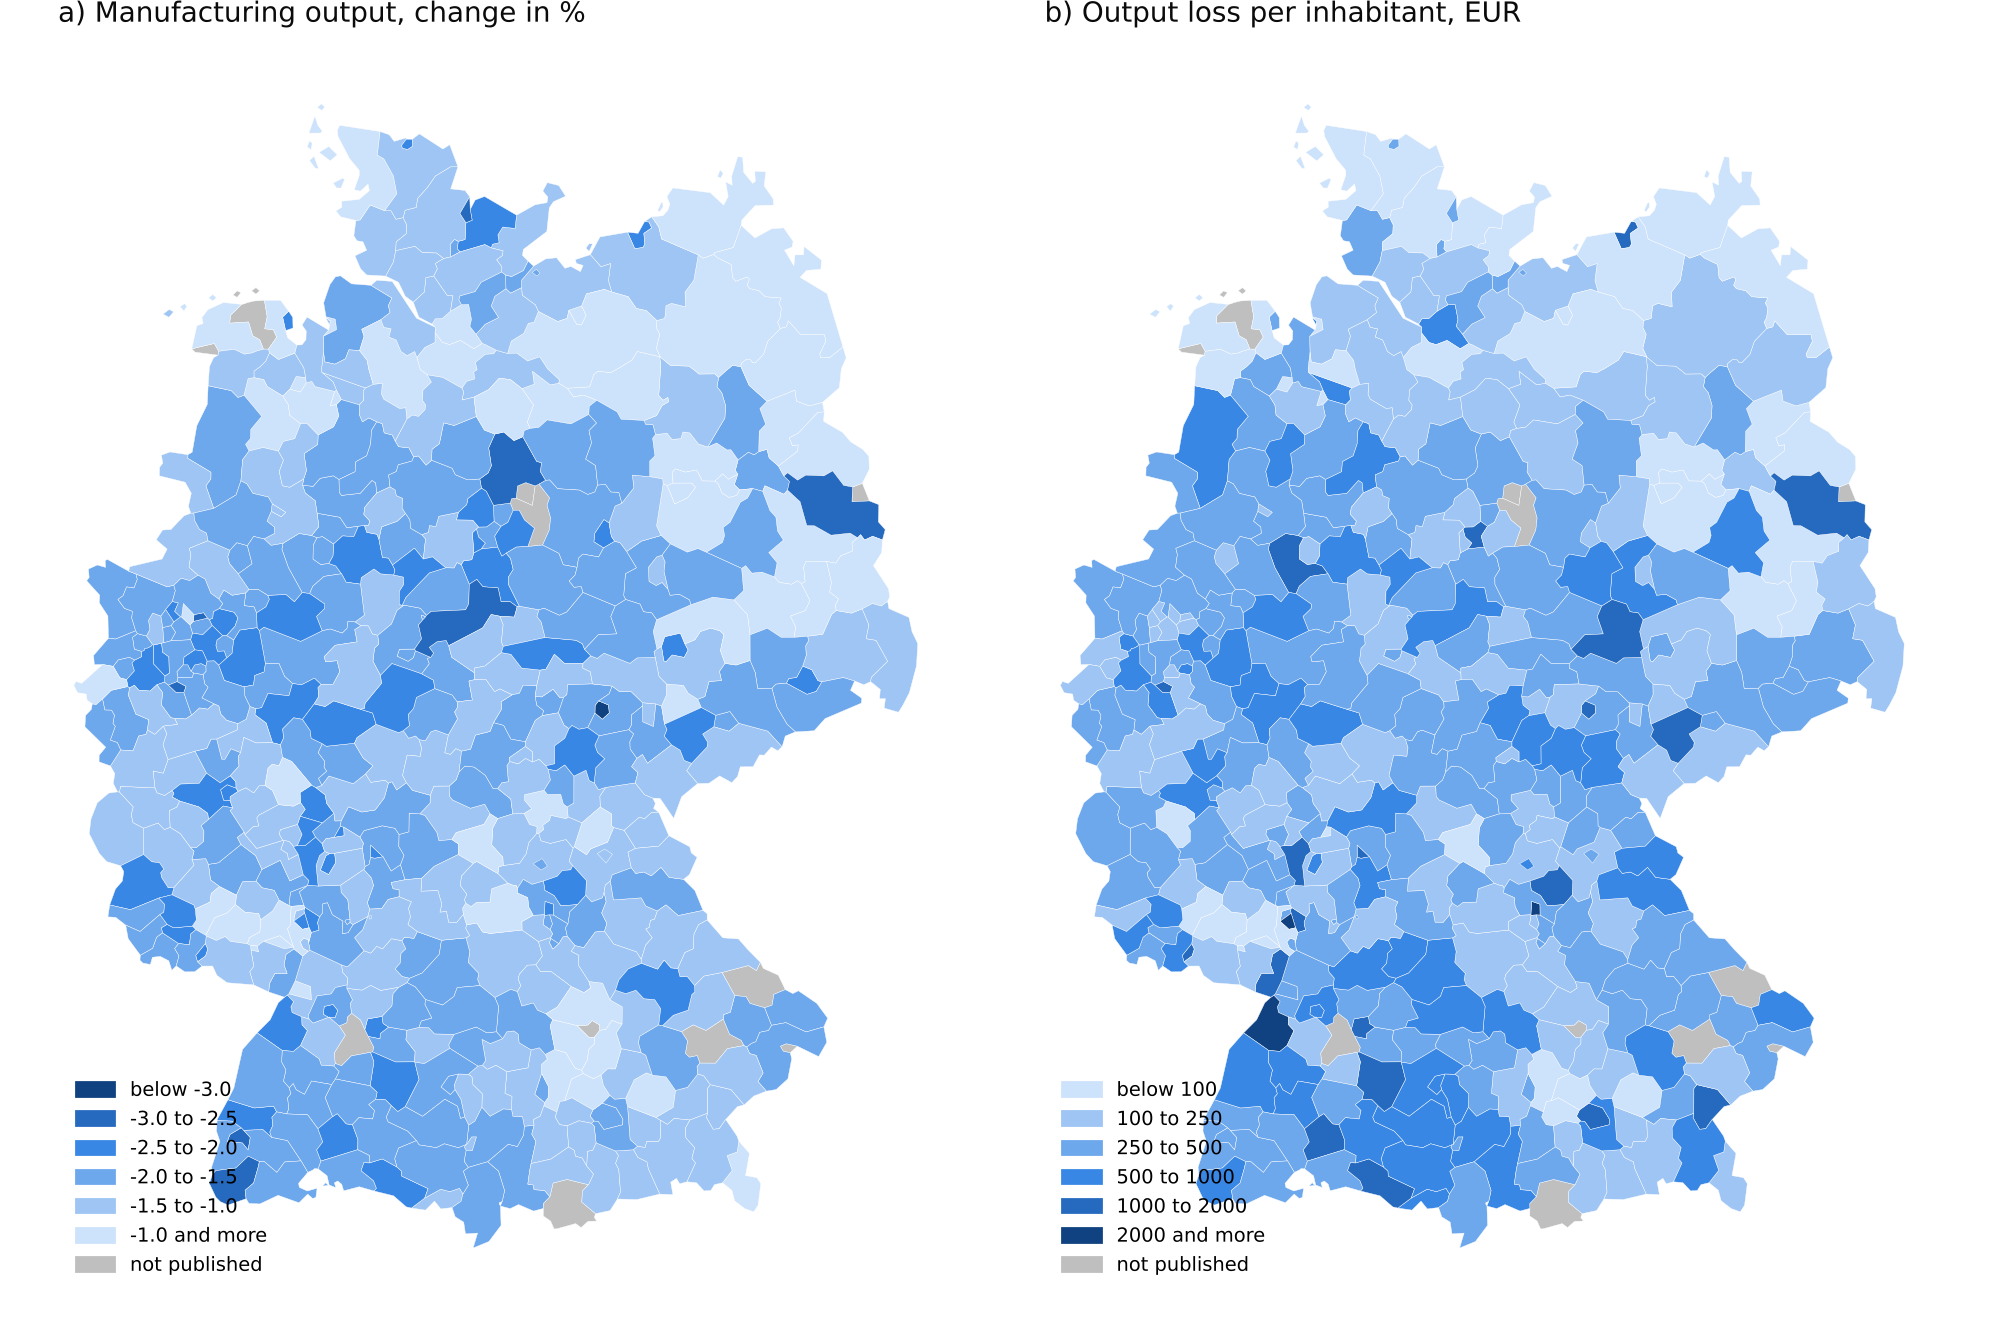
\includegraphics{figures_regional/fig1_map.png}
\caption{Manufacturing output change and output loss per inhabitant by
district, US tariffs of August 2026. Sources: own calculations;
Caliendo-Parro model, Eurostat, Regionaldatenbank 42111-04-02-4 (2024).
Grey: values not published.}
\end{figure}

The loss is concentrated. The most exposed fifth of districts carries 50
\% of it, the least exposed fifth 3 \% (Figure 2). Weighted by
population the curve is almost the same, so the concentration does not
come from small districts.

The 14 suppressed districts can be estimated. The totals of the
Regierungsbezirke (or of the Land) are published, so the suppressed
districts of each group are known together as a residual. For eight of
them sales are published and only foreign sales are suppressed. Where
sales are missing, smaller districts get their gross value added in the
secondary sector (national accounts of the Länder, 2022) times the
median ratio of sales to that value added in their Land, and the largest
plant location takes the rest; foreign sales follow sales times the
district's last published export ratio (script 89). With these values
the national loss rises to EUR 38.1 billion. The car locations move to
the top: Wolfsburg (EUR 13,600 per inhabitant, sales of EUR 83 billion),
Ingolstadt (6,300), Dingolfing-Landau (5,700) and Böblingen (3,200). The
rule can be tested on published districts (script 89). Masking the
largest district of a Regierungsbezirk together with one other district
and imputing both gives a median error of 5 \% in sales and 8 \% in the
loss per inhabitant for the large district, and a rank correlation of
0.97 between true and imputed losses. For the small district the median
error in the loss per inhabitant is 34 \%. Where only foreign sales are
missing, as for Böblingen, Emden or Heilbronn city, the median error is
below 4 \%, although the test uses the export ratio of the previous year
while Böblingen's last published ratio dates from 2009. The estimates
for Wolfsburg, Ingolstadt and Dingolfing-Landau, the dominant plants of
their groups, are therefore reasonably reliable; those for Helmstedt,
Garmisch-Partenkirchen and Regen are not. The tables and maps use the
published data, and Section 10 treats the imputation as a variant.

\begin{figure}
\centering
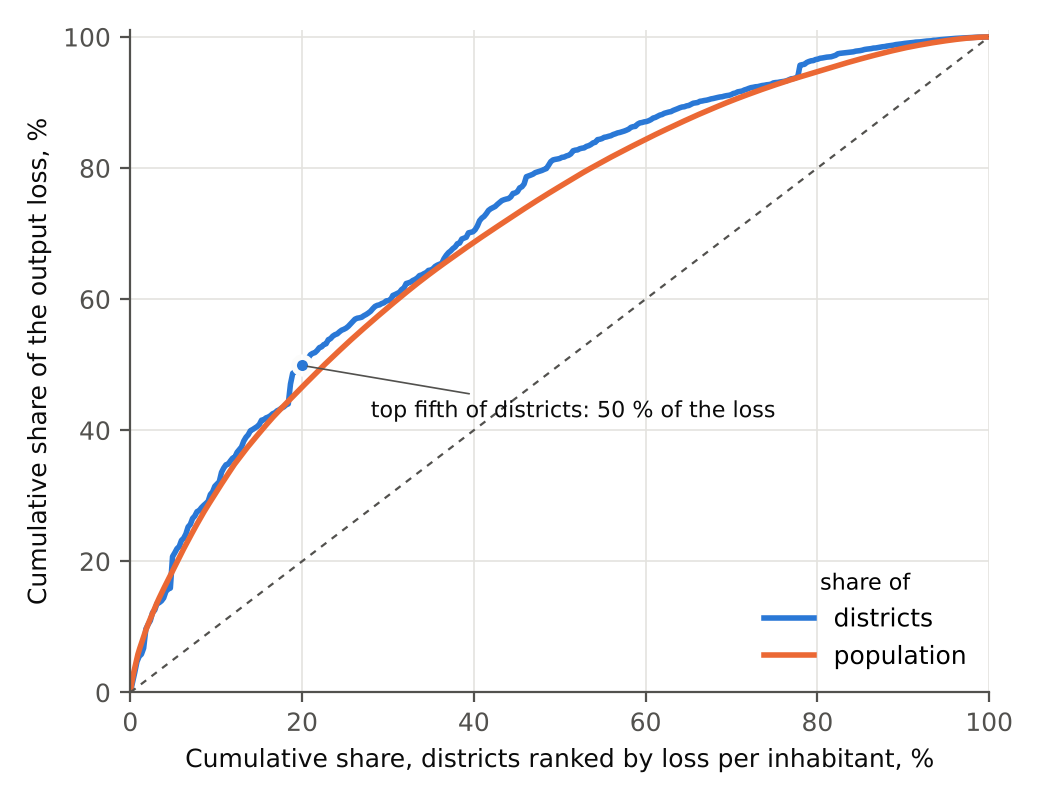
\includegraphics[width=0.7\textwidth,height=\textheight]{figures_regional/fig2_concentration.png}
\caption{Concentration of the output loss. Districts ranked by loss per
inhabitant; blue: share of districts, orange: share of population.}
\end{figure}

\hypertarget{who-is-exposed}{%
\section{6 Who is exposed}\label{who-is-exposed}}

Splitting the districts into five groups of equal size by loss per
inhabitant shows a clear profile (Table 1). The most exposed fifth (Q5)
has a GDP per head of EUR 61 thousand against 37 thousand in the least
exposed fifth (Q1), median earnings 20 \% higher, almost twice the
industry employment rate, a younger population and lower unemployment.
Across all districts the loss correlates most with industry employment
per working-age inhabitant (Figure 3).

\textbf{Table 1: Profile of districts by exposure to US tariffs
(quintiles of loss per inhabitant)}

\begingroup\small
\begin{longtable}[]{@{}
  >{\raggedright\arraybackslash}p{(\columnwidth - 10\tabcolsep) * \real{0.5455}}
  >{\raggedleft\arraybackslash}p{(\columnwidth - 10\tabcolsep) * \real{0.0909}}
  >{\raggedleft\arraybackslash}p{(\columnwidth - 10\tabcolsep) * \real{0.0909}}
  >{\raggedleft\arraybackslash}p{(\columnwidth - 10\tabcolsep) * \real{0.0909}}
  >{\raggedleft\arraybackslash}p{(\columnwidth - 10\tabcolsep) * \real{0.0909}}
  >{\raggedleft\arraybackslash}p{(\columnwidth - 10\tabcolsep) * \real{0.0909}}@{}}
\toprule\noalign{}
\begin{minipage}[b]{\linewidth}\raggedright
Indicator (population-weighted mean)
\end{minipage} & \begin{minipage}[b]{\linewidth}\raggedleft
Q1
\end{minipage} & \begin{minipage}[b]{\linewidth}\raggedleft
Q2
\end{minipage} & \begin{minipage}[b]{\linewidth}\raggedleft
Q3
\end{minipage} & \begin{minipage}[b]{\linewidth}\raggedleft
Q4
\end{minipage} & \begin{minipage}[b]{\linewidth}\raggedleft
Q5
\end{minipage} \\
\midrule\noalign{}
\endhead
\bottomrule\noalign{}
\endlastfoot
Output loss per inhabitant, EUR & 94 & 192 & 310 & 438 & 919 \\
GDP per head, EUR thousand (2022) & 37.2 & 40.5 & 44.3 & 44.7 & 60.6 \\
Median full-time earnings, EUR per month & 3,420 & 3,683 & 3,768 & 3,677
& 4,104 \\
Industry employees per 100 aged 15-64 & 12.0 & 14.2 & 16.7 & 20.7 &
22.6 \\
Employees with university degree, \% & 14.4 & 18.9 & 17.0 & 15.4 &
20.9 \\
Unemployment rate, \% & 6.0 & 6.2 & 5.9 & 5.1 & 5.5 \\
Mean age, years & 45.2 & 44.3 & 44.3 & 44.4 & 43.5 \\
Population change 2013-2023, \% & 3.6 & 3.4 & 3.3 & 3.3 & 3.7 \\
\end{longtable}
\endgroup


Source: BBSR (2025), INKAR; own calculations. Indicators 2023 unless
stated.

\begin{figure}
\centering
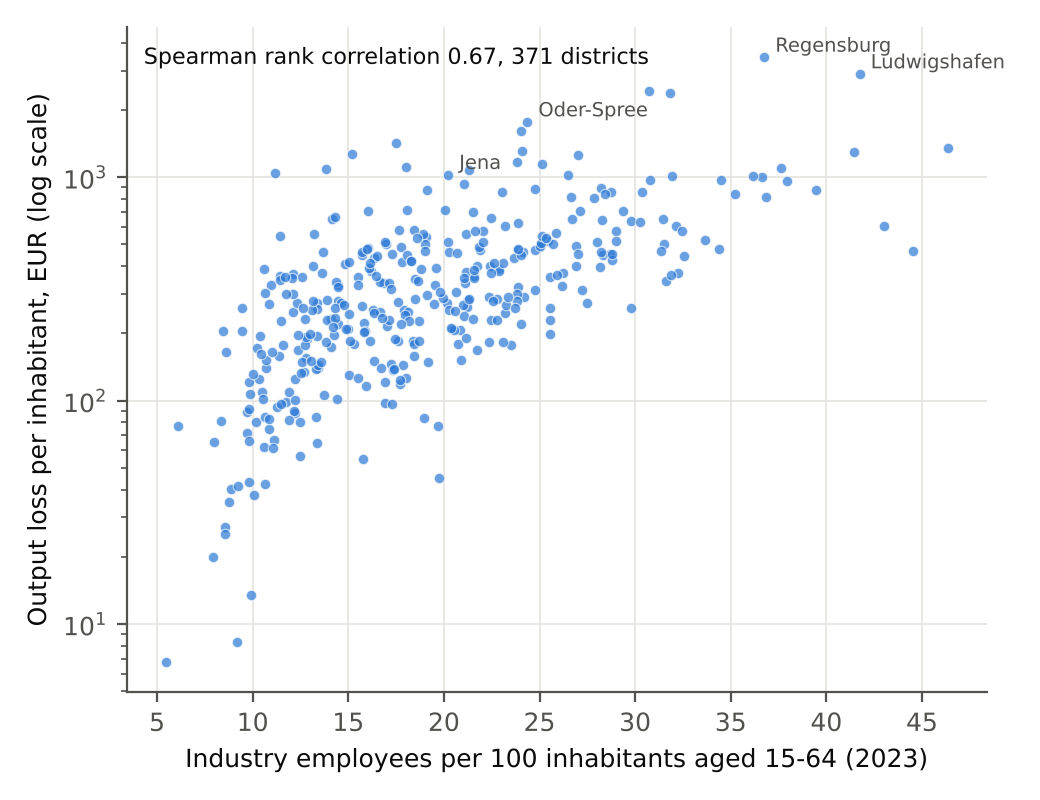
\includegraphics[width=0.7\textwidth,height=\textheight]{figures_regional/fig3_industry.png}
\caption{Output loss per inhabitant and industry employment rate by
district.}
\end{figure}

Regressions with Land fixed effects, robust standard errors and
standardised regressors (script 79) confirm the pattern. The share of
Gewerbesteuer in municipal tax capacity rises by 2.7 percentage points
per standard deviation of exposure (p = 0.007), controlling for earnings
and density.

\hypertarget{what-the-tariff-structure-adds}{%
\subsection{6.1 What the tariff structure
adds}\label{what-the-tariff-structure-adds}}

The loss per inhabitant is the product of two factors: manufacturing
sales per inhabitant and the percentage output loss, which carries the
tariff structure through the regional industry mix and the district
export ratio:

\[ \frac{V_k}{P_k} = \frac{U_k}{P_k}\, s_k, \qquad s_k = -\Delta Y_k . \]

Any shock proportional to manufacturing output would rank districts by
the first factor alone. A benchmark makes this explicit (script 91): a
uniform shock that lowers manufacturing output everywhere by the
national average of 1.65 \% has the same total loss as the tariffs. Its
ranking of districts by loss per inhabitant is almost identical to the
tariff ranking (rank correlation 0.90). In logarithms, manufacturing
intensity accounts for 69 \% of the variance of the loss per inhabitant
and the tariff-specific percentage shock for 31 \%.

The profile of Table 1 therefore mostly describes where German
manufacturing is. Figure 4 separates the two factors. Manufacturing
intensity carries the strong link with industry employment (rank
correlation 0.78) and the negative link with unemployment (−0.20). The
tariff-specific shock s\textsubscript{k} correlates only weakly with
industry employment (0.17), more with earnings (0.38) and GDP per head
(0.24), and slightly positively with unemployment (0.18) and the SGB II
rate (0.23). The last two links reflect cities: the shock is larger in
independent cities with high export ratios (median 1.69 \% against 1.46
\% in rural districts, rank correlation with density 0.36). With Land
fixed effects and density as control, s\textsubscript{k} is unrelated to
unemployment and the SGB II rate (p = 0.50 and 0.97), while one
percentage point more output loss goes with 4 \% higher earnings (p
\textless{} 0.001). Table 2 shows the raw profile by quintile of
s\textsubscript{k}.

\textbf{Table 2: Districts by tariff intensity (quintiles of the
percentage output loss)}

\begingroup\footnotesize
\begin{longtable}[]{@{}
  >{\raggedright\arraybackslash}p{(\columnwidth - 16\tabcolsep) * \real{0.1020}}
  >{\raggedleft\arraybackslash}p{(\columnwidth - 16\tabcolsep) * \real{0.1122}}
  >{\raggedleft\arraybackslash}p{(\columnwidth - 16\tabcolsep) * \real{0.0816}}
  >{\raggedleft\arraybackslash}p{(\columnwidth - 16\tabcolsep) * \real{0.1531}}
  >{\raggedleft\arraybackslash}p{(\columnwidth - 16\tabcolsep) * \real{0.1020}}
  >{\raggedleft\arraybackslash}p{(\columnwidth - 16\tabcolsep) * \real{0.1122}}
  >{\raggedleft\arraybackslash}p{(\columnwidth - 16\tabcolsep) * \real{0.1429}}
  >{\raggedleft\arraybackslash}p{(\columnwidth - 16\tabcolsep) * \real{0.0714}}
  >{\raggedleft\arraybackslash}p{(\columnwidth - 16\tabcolsep) * \real{0.1224}}@{}}
\toprule\noalign{}
\begin{minipage}[b]{\linewidth}\raggedright
Quintile
\end{minipage} & \begin{minipage}[b]{\linewidth}\raggedleft
Districts
\end{minipage} & \begin{minipage}[b]{\linewidth}\raggedleft
Output loss, \%
\end{minipage} & \begin{minipage}[b]{\linewidth}\raggedleft
Manufacturing sales per inhabitant, EUR thousand
\end{minipage} & \begin{minipage}[b]{\linewidth}\raggedleft
GDP per head, EUR thousand
\end{minipage} & \begin{minipage}[b]{\linewidth}\raggedleft
Median earnings, EUR
\end{minipage} & \begin{minipage}[b]{\linewidth}\raggedleft
Unemployment rate, \%
\end{minipage} & \begin{minipage}[b]{\linewidth}\raggedleft
SGB II rate, \%
\end{minipage} & \begin{minipage}[b]{\linewidth}\raggedleft
Population in C areas, \%
\end{minipage} \\
\midrule\noalign{}
\endhead
\bottomrule\noalign{}
\endlastfoot
1 & 78 & 0.85 & 24.9 & 43.4 & 3,516 & 6.0 & 8.2 & 28 \\
2 & 77 & 1.24 & 18.7 & 38.5 & 3,546 & 4.5 & 6.1 & 15 \\
3 & 77 & 1.52 & 27.3 & 43.5 & 3,712 & 4.9 & 6.9 & 9 \\
4 & 77 & 1.76 & 20.2 & 47.9 & 3,834 & 6.4 & 9.8 & 22 \\
5 & 77 & 2.21 & 34.1 & 53.7 & 4,016 & 6.2 & 9.3 & 13 \\
\end{longtable}
\endgroup


Source: own calculations; BBSR (2025), INKAR. Manufacturing sales of
establishments with 20 and more employees, 2024. Means weighted by
population.

\begin{figure}
\centering
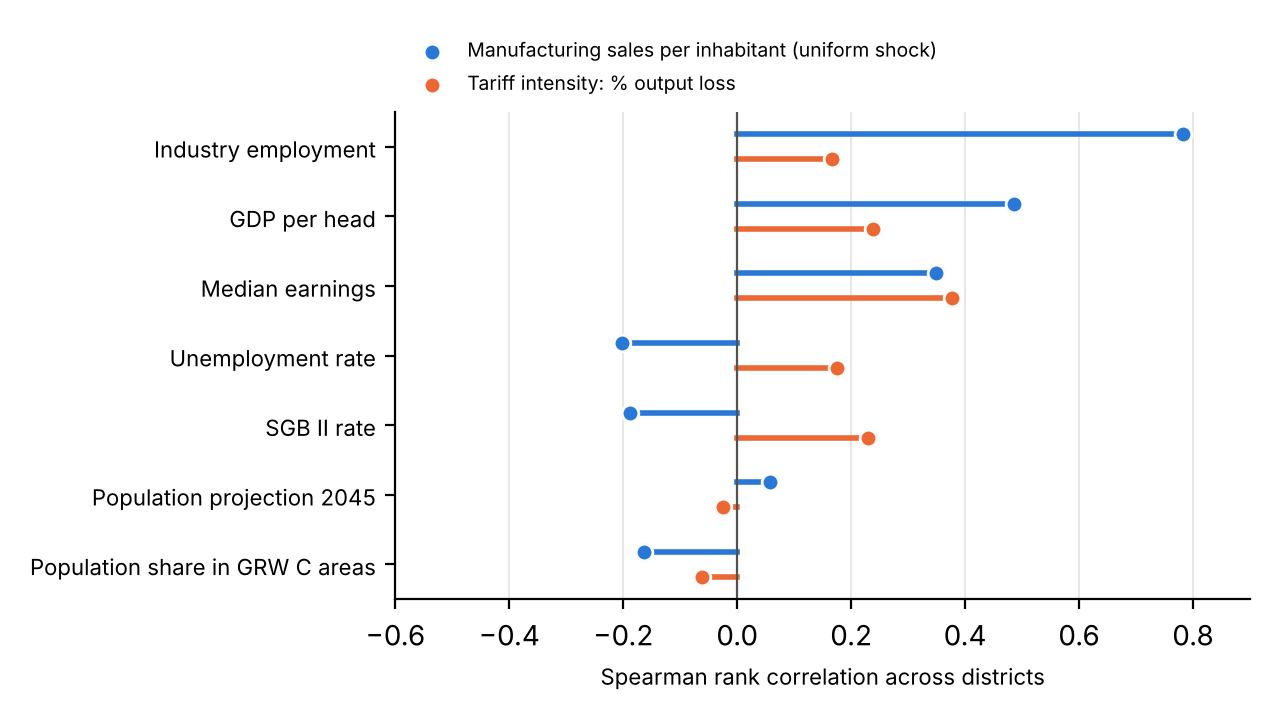
\includegraphics[width=0.8\textwidth,height=\textheight]{figures_regional/fig6_decomposition.png}
\caption{Rank correlations of the two factors of the loss per inhabitant
with district characteristics. Blue: manufacturing sales per inhabitant,
which alone ranks districts under a uniform shock; orange: the
tariff-specific percentage output loss.}
\end{figure}

What the tariff structure adds is concentration, not a different set of
regions. Under the benchmark the most exposed fifth of districts carries
45 \% of the loss, under the tariffs 50 \%. The share of the loss in GRW
C areas hardly changes (13.1 \% under the benchmark, 12.5 \% under the
tariffs). For policy this matters: the mismatch with regional aid is a
property of German industrial geography, and it would arise for almost
any shock to manufacturing.

\hypertarget{missing-links}{%
\subsection{6.2 Missing links}\label{missing-links}}

Several expected links are absent. Neither the change in the export
ratio since 2019 nor the energy intensity of the regional industry mix
explains where industry employment fell between 2019 and 2023.
Unemployment is slightly lower in exposed districts (5.5 \% against 6.0
\%), but INKAR has no vacancy totals that would show whether displaced
workers would find new jobs locally.

\hypertarget{local-business-tax}{%
\section{7 Local business tax}\label{local-business-tax}}

\hypertarget{the-channel}{%
\subsection{7.1 The channel}\label{the-channel}}

Gewerbesteuer is the main own tax of German municipalities, EUR 73
billion in 2023. Its base is business profit with add-backs; for firms
with plants in several municipalities it is apportioned by payroll (§ 29
GewStG). Prepayments follow the last assessment, so receipts react with
a lag. In the most exposed fifth of districts Gewerbesteuer brings EUR
1,269 per inhabitant, twice as much as in the least exposed fifth (EUR
599), and 80 \% of tax capacity against 60 \%.

\hypertarget{elasticity}{%
\subsection{7.2 Elasticity}\label{elasticity}}

To translate output into tax, the paper estimates the elasticity of
Gewerbesteuer per inhabitant to manufacturing sales per inhabitant in a
district panel for 2009 to 2023 (script 87):

\[ \ln G_{kt} = \beta \ln U_{kt} + \alpha_k + \delta_t + \varepsilon_{kt} , \]

with district effects α\textsubscript{k} and year effects
δ\textsubscript{t}, standard errors clustered by district. Year effects
remove the national cycle, so β measures the response to a
district-specific change in sales, which is the kind of variation the
regional allocation of the tariff loss creates. The apportionment of the
tax base by payroll is part of this reduced form.

The elasticity is about 0.2 and stable across specifications (Table 3,
Figure 5): 0.24 in levels, 0.18 with population weights, 0.17 for the
sum of current and two lagged changes in first differences, and 0.25 in
long differences between 2010-12 and 2021-23. In the most industrial
third of districts it is 0.43, twice that of the other two thirds. With
standard errors clustered by NUTS 2 region, which allows for regional
shocks, all estimates stay significant; the standard error of the levels
estimate rises from 0.047 to 0.054. In a placebo test next year's sales
add 0.08 while the current-year coefficient stays at 0.19. The lead is
insignificant with district clusters (standard error 0.045) and
marginally significant with regional clusters (0.037), which fits
persistent sales or anticipated changes; the current-year response is
more than twice as large.

\textbf{Table 3: Elasticity of Gewerbesteuer to manufacturing sales,
district panel 2009-2023}

\begingroup\small
\begin{longtable}[]{@{}
  >{\raggedright\arraybackslash}p{(\columnwidth - 8\tabcolsep) * \real{0.5306}}
  >{\raggedleft\arraybackslash}p{(\columnwidth - 8\tabcolsep) * \real{0.1224}}
  >{\raggedleft\arraybackslash}p{(\columnwidth - 8\tabcolsep) * \real{0.1020}}
  >{\raggedleft\arraybackslash}p{(\columnwidth - 8\tabcolsep) * \real{0.1020}}
  >{\raggedleft\arraybackslash}p{(\columnwidth - 8\tabcolsep) * \real{0.1429}}@{}}
\toprule\noalign{}
\begin{minipage}[b]{\linewidth}\raggedright
Model
\end{minipage} & \begin{minipage}[b]{\linewidth}\raggedleft
Elasticity
\end{minipage} & \begin{minipage}[b]{\linewidth}\raggedleft
Std. error, district clusters
\end{minipage} & \begin{minipage}[b]{\linewidth}\raggedleft
Std. error, NUTS 2 clusters
\end{minipage} & \begin{minipage}[b]{\linewidth}\raggedleft
Observations
\end{minipage} \\
\midrule\noalign{}
\endhead
\bottomrule\noalign{}
\endlastfoot
Levels, district and year effects & 0.239 & 0.047 & 0.054 & 5,777 \\
Levels, population-weighted & 0.180 & 0.049 & 0.055 & 5,777 \\
First differences, sum of lags 0 to 2 & 0.172 & 0.052 & 0.058 & 4,592 \\
Long difference 2010-12 to 2021-23, Land effects & 0.249 & 0.066 & 0.081
& 383 \\
Levels with next year's sales: current year & 0.191 & 0.051 & 0.059 &
5,384 \\
Levels with next year's sales: next year (placebo) & 0.079 & 0.045 &
0.037 & 5,384 \\
Levels, least industrial third & 0.205 & 0.072 & 0.072 & 1,913 \\
Levels, middle third & 0.173 & 0.062 & 0.055 & 1,980 \\
Levels, most industrial third & 0.426 & 0.123 & 0.151 & 1,884 \\
\end{longtable}
\endgroup


Source: BBSR (2025), INKAR; Regionaldatenbank 42111-04-02-4; own
calculations. Standard errors clustered by district (long difference:
heteroskedasticity-robust) and, as a check, by NUTS 2 region. First
differences exclude changes of more than 150 \% in tax and 100 \% in
sales.

\begin{figure}
\centering
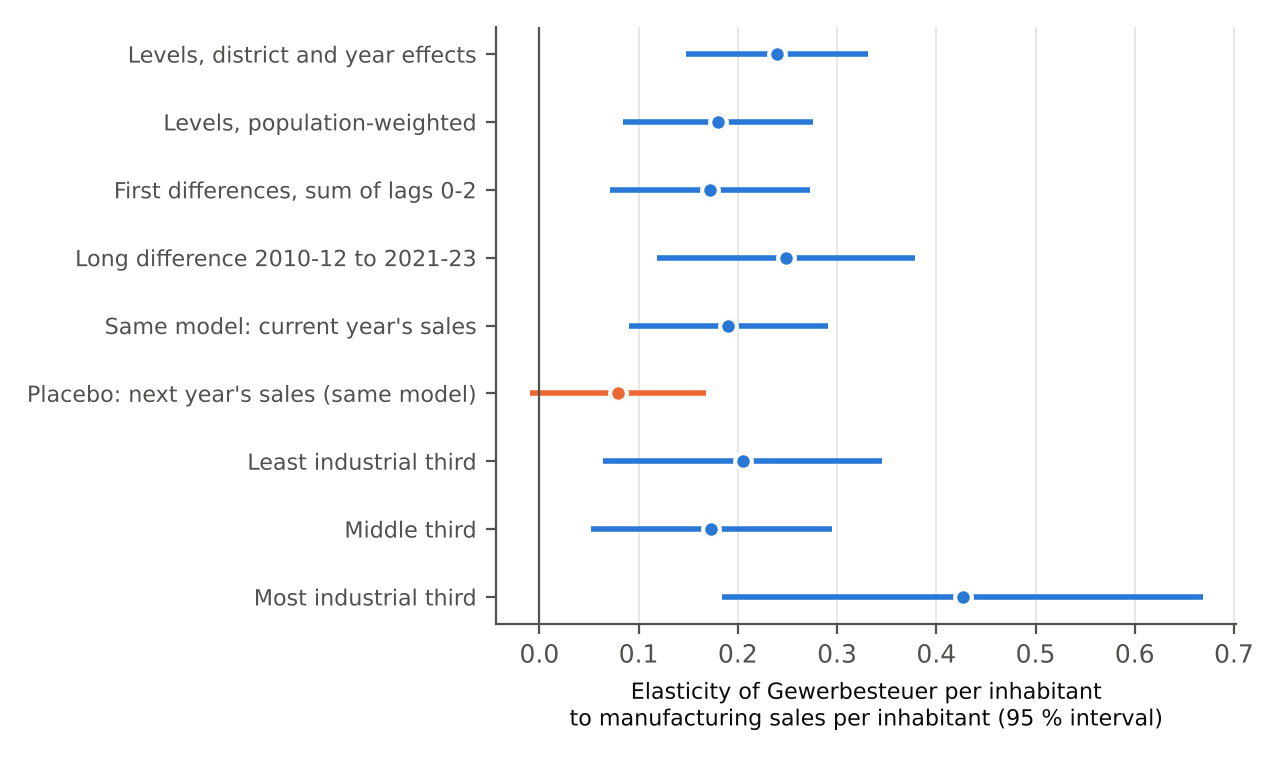
\includegraphics[width=0.8\textwidth,height=\textheight]{figures_regional/fig4_elasticity.png}
\caption{Elasticity of Gewerbesteuer to manufacturing sales, all
specifications, 95 \% intervals.}
\end{figure}

The district elasticity is far below the national one. In 2009
Gewerbesteuer fell by 21 \% while manufacturing sales fell by about 21
\%, an elasticity near one. A national shock lowers profits in all
sectors, through demand and supply chains, and through firms'
headquarters; a district-specific shock moves only the local plants'
share of profits. Because the tariff shock is national, the district
elasticity gives a lower bound and the national one an upper bound, and
the upper bound is at least as plausible as the lower.

\hypertarget{tax-loss}{%
\subsection{7.3 Tax loss}\label{tax-loss}}

Applying the tercile elasticities to the district output changes gives a
tax loss of EUR 0.30 billion a year, 0.4 \% of receipts (95 \% band 0.18
to 0.43 billion, from the larger of the district and regional standard
errors of the tercile estimates). A uniform elasticity of 0.24 gives
0.29 billion; an elasticity of one gives 1.2 billion. The loss rises
from EUR 1.3 per inhabitant in the least to EUR 6.6 in the most exposed
fifth (Table 4). With these elasticities even the most affected
municipalities lose less than 1 \% of their tax capacity, and with an
elasticity of one about four times as much: Coburg city (EUR 22 per
inhabitant), the district of Munich (20), Erlangen (18) and Regensburg
city (17). Places with a high output loss but low current profits, such
as Ludwigshafen, lose little tax. Of the tax loss 11 \% falls in GRW C
areas and 29 \% in C or D areas. With the imputed districts the loss is
EUR 0.31 billion; Böblingen, Wolfsburg and Dingolfing-Landau then lose
EUR 16 to 20 per inhabitant.

These are gross figures; three mechanisms reduce the net loss of
municipalities. A share of Gewerbesteuer goes to the federal government
and the Länder as a levy on the tax base (Gewerbesteuerumlage), under a
tenth of receipts at the usual municipal rates (Hebesätze) above 400 \%.
Lower tax capacity reduces the contributions that municipalities pay to
their district (Kreisumlage) and, in some Länder, to equalisation funds.
Municipalities below their fiscal need receive higher general grants
(Schlüsselzuweisungen) under the fiscal equalisation of their Land,
which replaces a large part of a loss in tax capacity. The exposed
municipalities are often fiscally strong and receive few such grants, so
they bear more of their loss than weaker places. Quantifying the net
effect requires the equalisation rules of each Land and is left for
further work.

\textbf{Table 4: Gewerbesteuer loss by exposure quintile, central
elasticities}

\begingroup\small
\begin{longtable}[]{@{}
  >{\raggedright\arraybackslash}p{(\columnwidth - 8\tabcolsep) * \real{0.1613}}
  >{\raggedleft\arraybackslash}p{(\columnwidth - 8\tabcolsep) * \real{0.2419}}
  >{\raggedleft\arraybackslash}p{(\columnwidth - 8\tabcolsep) * \real{0.1935}}
  >{\raggedleft\arraybackslash}p{(\columnwidth - 8\tabcolsep) * \real{0.2419}}
  >{\raggedleft\arraybackslash}p{(\columnwidth - 8\tabcolsep) * \real{0.1613}}@{}}
\toprule\noalign{}
\begin{minipage}[b]{\linewidth}\raggedright
Quintile
\end{minipage} & \begin{minipage}[b]{\linewidth}\raggedleft
Gewerbesteuer 2023, EUR per inhabitant
\end{minipage} & \begin{minipage}[b]{\linewidth}\raggedleft
Tax loss, EUR per inhabitant
\end{minipage} & \begin{minipage}[b]{\linewidth}\raggedleft
Tax loss, \% of Gewerbesteuer
\end{minipage} & \begin{minipage}[b]{\linewidth}\raggedleft
Tax loss, \% of tax capacity
\end{minipage} \\
\midrule\noalign{}
\endhead
\bottomrule\noalign{}
\endlastfoot
1 & 598 & −1.3 & −0.21 & −0.13 \\
2 & 725 & −2.3 & −0.31 & −0.20 \\
3 & 908 & −3.3 & −0.37 & −0.26 \\
4 & 849 & −4.0 & −0.49 & −0.34 \\
5 & 1,269 & −6.6 & −0.57 & −0.44 \\
\end{longtable}
\endgroup


Source: own calculations. Tax capacity (Steuerkraft) as defined by
INKAR, 2023.

\hypertarget{regional-aid-and-double-risks}{%
\section{8 Regional aid and double
risks}\label{regional-aid-and-double-risks}}

The GRW, the joint federal-state programme for regional economic
structure, supports investment in C areas (eligible under EU state aid
rules) and, with lower rates, in D areas. In C areas live 17 \% of the
population, in C or D areas 42 \%. They account for only 13 \% and 32 \%
of the output loss. In the most exposed fifth of districts 8 \% of the
population lives in C areas, in the least exposed fifth 27 \% (Table 5).
Of the twelve districts with the highest loss per inhabitant only
Oder-Spree is a C area.

\textbf{Table 5: Population in GRW aid areas by exposure quintile}

\begingroup\small
\begin{longtable}[]{@{}
  >{\raggedright\arraybackslash}p{(\columnwidth - 6\tabcolsep) * \real{0.2222}}
  >{\raggedleft\arraybackslash}p{(\columnwidth - 6\tabcolsep) * \real{0.2444}}
  >{\raggedleft\arraybackslash}p{(\columnwidth - 6\tabcolsep) * \real{0.2667}}
  >{\raggedleft\arraybackslash}p{(\columnwidth - 6\tabcolsep) * \real{0.2667}}@{}}
\toprule\noalign{}
\begin{minipage}[b]{\linewidth}\raggedright
Quintile
\end{minipage} & \begin{minipage}[b]{\linewidth}\raggedleft
Districts
\end{minipage} & \begin{minipage}[b]{\linewidth}\raggedleft
Population in C areas, \%
\end{minipage} & \begin{minipage}[b]{\linewidth}\raggedleft
Population in C or D areas, \%
\end{minipage} \\
\midrule\noalign{}
\endhead
\bottomrule\noalign{}
\endlastfoot
1 & 78 & 27 & 67 \\
2 & 77 & 26 & 46 \\
3 & 77 & 17 & 41 \\
4 & 77 & 12 & 43 \\
5 & 77 & 8 & 23 \\
\end{longtable}
\endgroup


Source: BBSR, Raumgliederungen Referenz 2023; own calculations.
Municipalities with split status counted in equal parts.

On average the shock does not hit weak districts, but some combine a
high loss with a second risk. Of the 77 districts in the most exposed
fifth, 26 either shrink by more than 5 \% to 2045 in the BBSR projection
or have an SGB II rate in the top fifth of districts (10.2 \% or more);
four have both (Appendix Table A2). Two groups stand out: western
industrial cities with high welfare rates, such as Ludwigshafen,
Leverkusen, Mannheim and Krefeld, and shrinking industrial districts in
eastern Germany, the Saarland and the Sauerland, such as Zwickau,
Saalekreis, Saarlouis and Olpe. Eight of the 26 are fully or mainly C
areas, seven D areas, and eleven lie outside any aid area.

\hypertarget{labour-market-regions}{%
\section{9 Labour market regions}\label{labour-market-regions}}

Districts are where plants are, not where all their workers live. Many
plants draw commuters from neighbouring districts, so a district-level
loss overstates the concentration of income losses. The BBSR groups the
400 districts into 223 labour market regions by commuting flows. Summing
the losses (including the imputed districts) over these regions (script
90) gives a median loss of EUR 320 per inhabitant.

The concentration falls but stays high. The most exposed fifth of labour
market regions carries 47 \% of the loss, against 55 \% for the most
exposed fifth of districts with the same data; the coefficient of
variation of the loss per inhabitant falls from 1.9 to 1.1. The leading
regions are Dingolfing-Landau (EUR 5,700 per inhabitant), Wolfsburg
(2,000, seven districts), Baden-Baden (2,000), Ingolstadt (1,900),
Frankfurt (Oder) with Oder-Spree (1,400) and Tuttlingen (1,300) (Figure
6).

\textbf{Table 6: Labour market regions by exposure to US tariffs
(quintiles of loss per inhabitant)}

\begingroup\footnotesize
\begin{longtable}[]{@{}
  >{\raggedright\arraybackslash}p{(\columnwidth - 14\tabcolsep) * \real{0.1111}}
  >{\raggedleft\arraybackslash}p{(\columnwidth - 14\tabcolsep) * \real{0.1000}}
  >{\raggedleft\arraybackslash}p{(\columnwidth - 14\tabcolsep) * \real{0.1333}}
  >{\raggedleft\arraybackslash}p{(\columnwidth - 14\tabcolsep) * \real{0.1111}}
  >{\raggedleft\arraybackslash}p{(\columnwidth - 14\tabcolsep) * \real{0.1222}}
  >{\raggedleft\arraybackslash}p{(\columnwidth - 14\tabcolsep) * \real{0.1556}}
  >{\raggedleft\arraybackslash}p{(\columnwidth - 14\tabcolsep) * \real{0.1333}}
  >{\raggedleft\arraybackslash}p{(\columnwidth - 14\tabcolsep) * \real{0.1333}}@{}}
\toprule\noalign{}
\begin{minipage}[b]{\linewidth}\raggedright
Quintile
\end{minipage} & \begin{minipage}[b]{\linewidth}\raggedleft
Regions
\end{minipage} & \begin{minipage}[b]{\linewidth}\raggedleft
Loss, EUR per inhabitant
\end{minipage} & \begin{minipage}[b]{\linewidth}\raggedleft
GDP per head, EUR thousand
\end{minipage} & \begin{minipage}[b]{\linewidth}\raggedleft
Industry employees per 100 aged 15-64
\end{minipage} & \begin{minipage}[b]{\linewidth}\raggedleft
Unemployment rate, \%
\end{minipage} & \begin{minipage}[b]{\linewidth}\raggedleft
Population in C areas, \%
\end{minipage} & \begin{minipage}[b]{\linewidth}\raggedleft
Population in C or D areas, \%
\end{minipage} \\
\midrule\noalign{}
\endhead
\bottomrule\noalign{}
\endlastfoot
1 & 45 & 130 & 39.6 & 11.7 & 7.5 & 45 & 78 \\
2 & 44 & 240 & 39.5 & 15.5 & 6.1 & 23 & 63 \\
3 & 45 & 343 & 44.8 & 16.7 & 5.9 & 15 & 41 \\
4 & 44 & 472 & 48.9 & 18.8 & 5.4 & 10 & 30 \\
5 & 45 & 927 & 55.1 & 22.3 & 4.5 & 6 & 17 \\
\end{longtable}
\endgroup


Source: BBSR (2025), INKAR and Raumgliederungen Referenz 2023; own
calculations including the imputed districts. Means weighted by
population.

The profile is the same as for districts, and in part sharper (Table 6).
GDP per head rises from EUR 40 thousand in the least to 55 thousand in
the most exposed fifth, unemployment falls from 7.5 \% to 4.5 \%. The
rank correlation of the loss with industry employment is 0.58, with GDP
per head 0.54, with earnings 0.50 and with unemployment −0.28. The
overlap with regional aid is even smaller: 6 \% of the population in the
most exposed fifth of regions lives in C areas, 44 \% in the least
exposed fifth, and 11 \% of the loss falls in C areas.

\begin{figure}
\centering
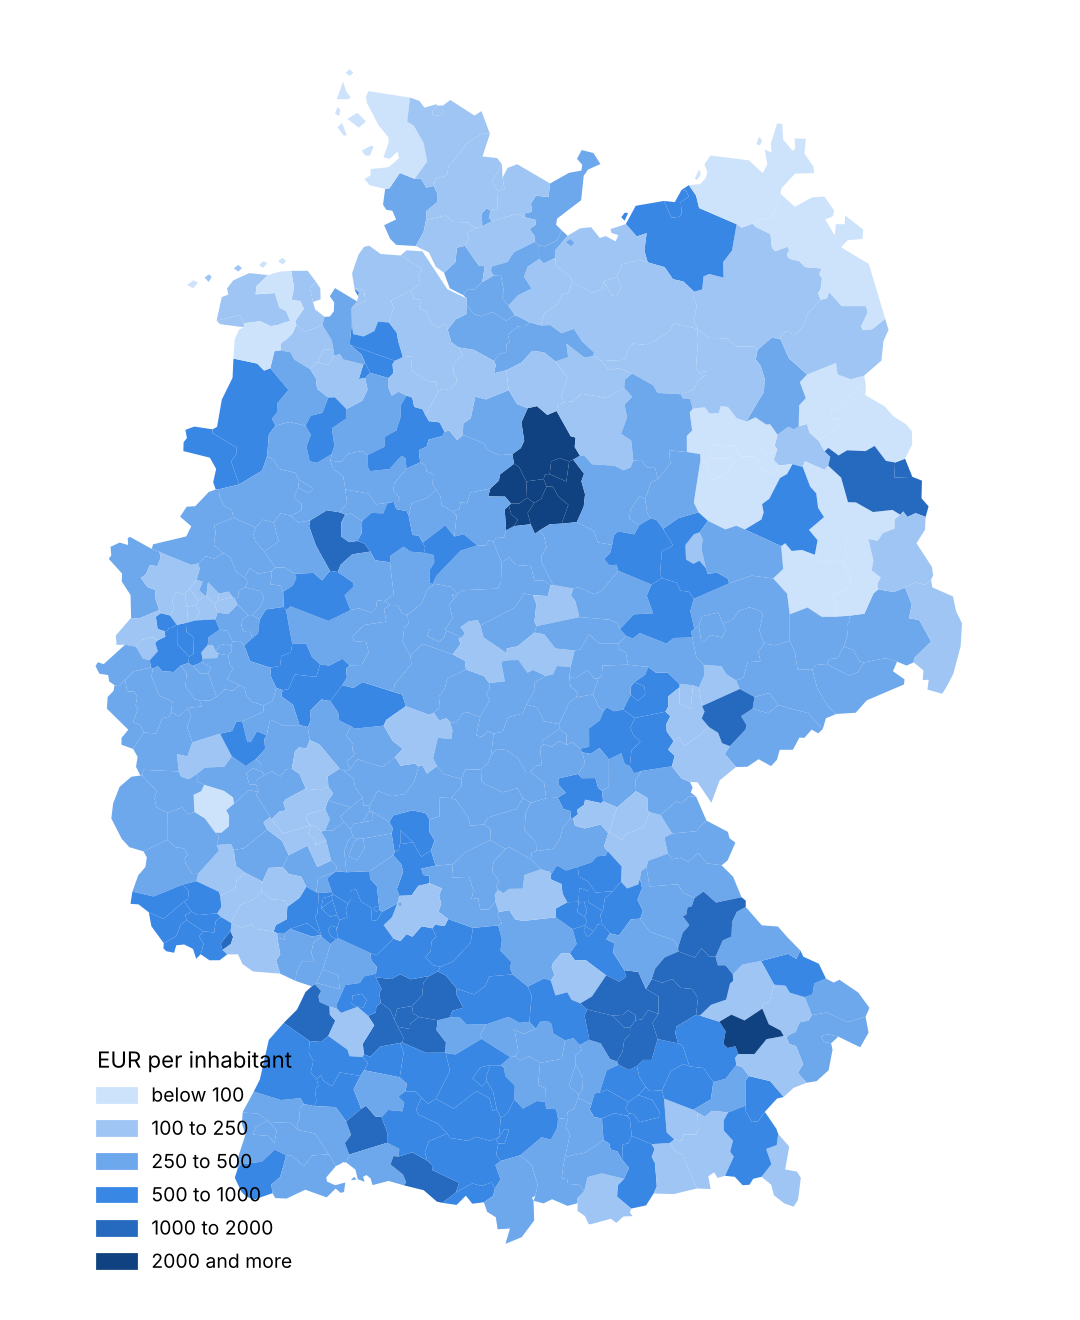
\includegraphics[width=0.6\textwidth,height=\textheight]{figures_regional/fig5_amr_map.png}
\caption{Output loss per inhabitant by labour market region, including
imputed districts. Each district shows the value of its labour market
region.}
\end{figure}

\hypertarget{robustness}{%
\section{10 Robustness}\label{robustness}}

The district allocation rests on assumptions that cannot be tested
directly with published data. Eight variants change one assumption at a
time (script 86; Table 7):

\begin{enumerate}
\def\labelenumi{\arabic{enumi}.}
\tightlist
\item
  Export ratio and sales of 2019, before Covid and the tariffs.
\item
  Export ratio and sales averaged over 2022 to 2024.
\item
  No scaling by the export ratio: every district takes its region's
  shock.
\item
  Half of the shock through exports, half proportional to output:
  m\textsubscript{r} · (0.5 + 0.5 q\textsubscript{k} /
  q\textsubscript{r}).
\item
  The regional loss allocated by industry employment times export ratio
  instead of sales times export ratio, which removes differences in
  productivity.
\item
  The tariff schedule after the framework deals of September 2025.
\item
  The August 2026 schedule with EU retaliation.
\item
  The baseline plus the 14 suppressed districts, imputed as in Section
  5.
\end{enumerate}

\textbf{Table 7: Robustness of the district results}

\begingroup\footnotesize
\begin{longtable}[]{@{}
  >{\raggedright\arraybackslash}p{(\columnwidth - 16\tabcolsep) * \real{0.3897}}
  >{\raggedleft\arraybackslash}p{(\columnwidth - 16\tabcolsep) * \real{0.0809}}
  >{\raggedleft\arraybackslash}p{(\columnwidth - 16\tabcolsep) * \real{0.0515}}
  >{\raggedleft\arraybackslash}p{(\columnwidth - 16\tabcolsep) * \real{0.0735}}
  >{\raggedleft\arraybackslash}p{(\columnwidth - 16\tabcolsep) * \real{0.0515}}
  >{\raggedleft\arraybackslash}p{(\columnwidth - 16\tabcolsep) * \real{0.0882}}
  >{\raggedleft\arraybackslash}p{(\columnwidth - 16\tabcolsep) * \real{0.0588}}
  >{\raggedleft\arraybackslash}p{(\columnwidth - 16\tabcolsep) * \real{0.1103}}
  >{\raggedleft\arraybackslash}p{(\columnwidth - 16\tabcolsep) * \real{0.0956}}@{}}
\toprule\noalign{}
\begin{minipage}[b]{\linewidth}\raggedright
Variant
\end{minipage} & \begin{minipage}[b]{\linewidth}\raggedleft
Districts
\end{minipage} & \begin{minipage}[b]{\linewidth}\raggedleft
Loss, EUR bn
\end{minipage} & \begin{minipage}[b]{\linewidth}\raggedleft
Rank corr. with baseline
\end{minipage} & \begin{minipage}[b]{\linewidth}\raggedleft
Top fifth kept, \%
\end{minipage} & \begin{minipage}[b]{\linewidth}\raggedleft
Rank corr. with industry employment
\end{minipage} & \begin{minipage}[b]{\linewidth}\raggedleft
Loss in C areas, \%
\end{minipage} & \begin{minipage}[b]{\linewidth}\raggedleft
Gewerbesteuer Q5/Q1
\end{minipage} & \begin{minipage}[b]{\linewidth}\raggedleft
Double-risk districts (in baseline)
\end{minipage} \\
\midrule\noalign{}
\endhead
\bottomrule\noalign{}
\endlastfoot
Baseline (export ratio 2024) & 386 & 34.0 & 1.00 & 100 & 0.67 & 13 &
2.12 & 26 (26) \\
Export ratio and sales 2019 & 376 & 28.9 & 0.96 & 83 & 0.69 & 12 & 1.75
& 25 (22) \\
Export ratio and sales 2022-2024 & 380 & 33.8 & 0.99 & 95 & 0.68 & 13 &
1.93 & 24 (24) \\
No export ratio (NUTS 2 mix only) & 386 & 34.0 & 0.92 & 83 & 0.78 & 13 &
1.84 & 22 (21) \\
Half exports, half output & 386 & 34.0 & 0.98 & 90 & 0.74 & 13 & 1.83 &
22 (21) \\
Employment instead of sales & 371 & 33.6 & 0.87 & 69 & 0.74 & 13 & 1.74
& 18 (14) \\
Scenario framework deals Sept 2025 & 386 & 44.9 & 0.98 & 94 & 0.70 & 12
& 1.86 & 24 (23) \\
Scenario with EU retaliation & 386 & 28.3 & 1.00 & 97 & 0.69 & 12 & 1.86
& 25 (24) \\
With imputed values for the 14 suppressed districts & 400 & 38.1 & 0.99
& 92 & 0.68 & 11 & 2.16 & 27 (25) \\
\end{longtable}
\endgroup


Source: own calculations. Variants 3 to 5 keep regional totals, so the
national loss is unchanged; variants 1, 2 and 5 cover fewer districts
because more values are suppressed; variant 8 covers all 400.

The ranking of districts barely changes: the rank correlation with the
baseline lies between 0.87 (employment weights) and 1.00 (retaliation).
Between 69 \% and 97 \% of the baseline top fifth stay in the top fifth.
The profile holds in every variant: the rank correlation with industry
employment lies between 0.67 and 0.78, the share of the loss in C areas
between 11 \% and 13 \%, and Gewerbesteuer per inhabitant in the top
fifth is 1.7 to 2.2 times that of the bottom fifth. The double-risk list
is less stable: 18 to 27 districts per variant, 14 to 25 of them in the
baseline list. Forty-two districts are in the top fifth under all seven
sales-based variants with published data (Appendix C).

\hypertarget{limitations}{%
\section{11 Limitations}\label{limitations}}

The allocation inherits the regional industry mix; within-region
variation comes only from the export ratio. A district with a car plant
in a machinery region is assigned the machinery region's mix. Employment
by industry division and district from the Federal Employment Agency
would remove this weakness. The export ratio covers establishments with
20 and more employees, and the 14 suppressed districts include some of
the largest car plants; their imputation rests on regional residuals and
assumed ratios of sales to value added. Foreign sales cover all
destinations, so districts with a high US share are understated and
districts selling mainly within the EU overstated. The model gives a
long-run, first-round effect without spillovers between districts
through supply chains or labour mobility; labour market regions (Section
9) capture commuting, not supplier links. Associations with district
characteristics are not causal, and the tax figures are gross of fiscal
equalisation. Finally, the double-risk list depends on thresholds.

\hypertarget{policy-conclusions}{%
\section{12 Policy conclusions}\label{policy-conclusions}}

The US tariff shock mainly hits economically strong districts outside
the regional aid map, largely because German manufacturing is located
there. Instruments of regional structural policy therefore reach only a
small part of the exposure. Three conclusions follow.

First, the fiscal risk for municipalities should be monitored, but it is
limited. The estimated gross loss of Gewerbesteuer is EUR 0.3 to 1.2
billion a year, between 1 \% and 4 \% of tax capacity in the most
affected places, and fiscal equalisation reduces the net loss of weaker
municipalities more than that of strong ones. An early warning through
the tax estimate and the Länder fits better than new support programmes.

Second, the 26 districts with a double risk deserve separate attention.
For the eleven outside any aid area, mainly western industrial cities,
the options are network and skills programmes or a change to the aid map
for the period from 2028.

Third, the data need improving. The largest gap is the confidential
industry mix of districts. A special evaluation of the employment
statistics by industry division and district would sharpen the
estimates, and the US share of foreign sales by Land would separate US
exposure from general export orientation.

\hypertarget{references}{%
\section{References}\label{references}}

Autor, D. H., D. Dorn and G. H. Hanson (2013), The China Syndrome: Local
Labor Market Effects of Import Competition in the United States,
\emph{American Economic Review}, 103(6), 2121-2168.

BBSR, Bundesinstitut für Bau-, Stadt- und Raumforschung (2025),
\emph{INKAR: Indikatoren und Karten zur Raum- und Stadtentwicklung},
edition 2025, Bonn.

Borusyak, K., P. Hull and X. Jaravel (2022), Quasi-Experimental
Shift-Share Research Designs, \emph{Review of Economic Studies}, 89(1),
181-213.

Caliendo, L. and F. Parro (2015), Estimates of the Trade and Welfare
Effects of NAFTA, \emph{Review of Economic Studies}, 82(1), 1-44.

Dauth, W., S. Findeisen and J. Suedekum (2014), The Rise of the East and
the Far East: German Labor Markets and Trade Integration, \emph{Journal
of the European Economic Association}, 12(6), 1643-1675.

Dekle, R., J. Eaton and S. Kortum (2008), Global Rebalancing with
Gravity: Measuring the Burden of Adjustment, \emph{IMF Staff Papers},
55(3), 511-540.

Dippel, C., R. Gold, S. Heblich and R. Pinto (2022), The Effect of Trade
on Workers and Voters, \emph{Economic Journal}, 132(641), 199-217.

Fajgelbaum, P. D., P. K. Goldberg, P. J. Kennedy and A. K. Khandelwal
(2020), The Return to Protectionism, \emph{Quarterly Journal of
Economics}, 135(1), 1-55.

Fontagné, L., H. Guimbard and G. Orefice (2022), Tariff-Based
Product-Level Trade Elasticities, \emph{Journal of International
Economics}, 137, 103593.

Goldsmith-Pinkham, P., I. Sorkin and H. Swift (2020), Bartik
Instruments: What, When, Why, and How, \emph{American Economic Review},
110(8), 2586-2624.

Guimbard, H. (2026), \emph{US applied tariffs 2025-26}, CEPII database,
Paris.

Hungerland, W.-F. (2026), Complexity, Gravity and Scenarios: An Open
Monitor of Germany's Trade Position, draft.

OECD (2025), \emph{Inter-Country Input-Output Tables}, 2025 edition
(2016 to 2022), Paris.

\hypertarget{appendix-a-data}{%
\section{Appendix A: Data}\label{appendix-a-data}}

\textbf{Table A1: Data sources}

\begin{longtable}[]{@{}
  >{\raggedright\arraybackslash}p{(\columnwidth - 4\tabcolsep) * \real{0.3333}}
  >{\raggedright\arraybackslash}p{(\columnwidth - 4\tabcolsep) * \real{0.3333}}
  >{\raggedright\arraybackslash}p{(\columnwidth - 4\tabcolsep) * \real{0.3333}}@{}}
\toprule\noalign{}
\begin{minipage}[b]{\linewidth}\raggedright
Source
\end{minipage} & \begin{minipage}[b]{\linewidth}\raggedright
Content
\end{minipage} & \begin{minipage}[b]{\linewidth}\raggedright
Use
\end{minipage} \\
\midrule\noalign{}
\endhead
\bottomrule\noalign{}
\endlastfoot
OECD ICIO 2025 & Input-output tables 2022, 81 economies, 50 sectors &
Model baseline \\
CEPII US applied tariffs (Guimbard 2026) & US tariffs by origin, HS6 and
date, 2025-2026 & Tariff shock \\
ProTEE 0.1 & Trade elasticities by HS6 & Sector elasticities \\
Eurostat sbs\_r\_nuts2021 & Persons employed by NACE division and NUTS 2
region & Regional industry mix \\
Regionaldatenbank 42111-04-02-4 & Sales and foreign sales of
manufacturing, establishments 20+, districts, 2009-2024 & Export ratio,
sales, tax panel \\
INKAR 2025 (BBSR) & District indicators, 1995-2023, projection to 2045 &
Profile, Gewerbesteuer, risks \\
BBSR Raumgliederungen Referenz 2023 & GRW status of each municipality &
Aid areas \\
Destatis district list, 31.12.2024; GISCO NUTS 2024 & District keys,
population, geometries & Matching, maps \\
\end{longtable}

\textbf{Table A2: Districts with high loss and a second risk}

\begingroup\footnotesize
\begin{longtable}[]{@{}
  >{\raggedright\arraybackslash}p{(\columnwidth - 12\tabcolsep) * \real{0.2885}}
  >{\raggedleft\arraybackslash}p{(\columnwidth - 12\tabcolsep) * \real{0.1154}}
  >{\raggedleft\arraybackslash}p{(\columnwidth - 12\tabcolsep) * \real{0.1154}}
  >{\raggedleft\arraybackslash}p{(\columnwidth - 12\tabcolsep) * \real{0.0673}}
  >{\raggedleft\arraybackslash}p{(\columnwidth - 12\tabcolsep) * \real{0.2212}}
  >{\raggedleft\arraybackslash}p{(\columnwidth - 12\tabcolsep) * \real{0.0769}}
  >{\raggedleft\arraybackslash}p{(\columnwidth - 12\tabcolsep) * \real{0.1154}}@{}}
\toprule\noalign{}
\begin{minipage}[b]{\linewidth}\raggedright
District
\end{minipage} & \begin{minipage}[b]{\linewidth}\raggedleft
Loss, EUR per inhabitant
\end{minipage} & \begin{minipage}[b]{\linewidth}\raggedleft
Population 2022-2045, \%
\end{minipage} & \begin{minipage}[b]{\linewidth}\raggedleft
SGB II rate, \%
\end{minipage} & \begin{minipage}[b]{\linewidth}\raggedleft
Second risk
\end{minipage} & \begin{minipage}[b]{\linewidth}\raggedleft
GRW status
\end{minipage} & \begin{minipage}[b]{\linewidth}\raggedleft
Tax loss, EUR per inhabitant
\end{minipage} \\
\midrule\noalign{}
\endhead
\bottomrule\noalign{}
\endlastfoot
Ludwigshafen am Rhein (city) & 2,902 & +4.2 & 13.5 & poverty & none &
−5.6 \\
Schweinfurt (city) & 2,042 & −3.7 & 10.6 & poverty & none & −10.8 \\
Leverkusen (city) & 1,424 & −1.1 & 12.3 & poverty & none & −6.2 \\
Mannheim (city) & 1,314 & +3.5 & 11.3 & poverty & none & −12.3 \\
Salzgitter (city) & 1,290 & −8.1 & 15.8 & shrinking and poverty & none &
−4.2 \\
Saalekreis & 1,073 & −14.2 & 8.5 & shrinking & C & −10.8 \\
Zwickau & 1,027 & −19.6 & 7.2 & shrinking & C & −5.0 \\
Olpe & 962 & −9.5 & 5.2 & shrinking & none & −8.7 \\
Holzminden & 897 & −6.8 & 10.4 & shrinking and poverty & D & −5.8 \\
Pforzheim (city) & 875 & −0.9 & 10.5 & poverty & none & −7.5 \\
Märkischer Kreis & 863 & −8.4 & 9.9 & shrinking & D & −7.8 \\
Saarpfalz-Kreis & 841 & −9.8 & 7.1 & shrinking & D & −6.7 \\
Bremen (city) & 826 & −2.5 & 16.3 & poverty & D & −3.1 \\
Siegen-Wittgenstein & 819 & −7.2 & 8.4 & shrinking & none & −9.0 \\
Krefeld (city) & 716 & −2.7 & 14.7 & poverty & none & −3.1 \\
Saarlouis & 713 & −10.4 & 7.7 & shrinking & C & −4.5 \\
Remscheid (city) & 640 & −4.9 & 12.0 & poverty & C & −6.8 \\
Anhalt-Bitterfeld & 604 & −20.1 & 10.7 & shrinking and poverty & C &
−2.3 \\
Tirschenreuth & 602 & −9.4 & 3.5 & shrinking & C & −10.0 \\
Saalfeld-Rudolstadt & 575 & −22.0 & 7.6 & shrinking & C & −7.1 \\
Ilm-Kreis & 563 & −12.2 & 7.8 & shrinking & D & −3.9 \\
St.~Wendel & 555 & −13.2 & 5.8 & shrinking & D & −2.0 \\
Hamburg & 555 & +7.5 & 12.2 & poverty & none & −3.1 \\
Köln (city) & 545 & +5.9 & 13.5 & poverty & none & −6.8 \\
Ennepe-Ruhr-Kreis & 542 & −3.6 & 10.8 & poverty & D & −2.9 \\
Salzlandkreis & 535 & −20.6 & 12.4 & shrinking and poverty & C & −1.8 \\
\end{longtable}
\endgroup


Source: own calculations. Second risk: projected population change
2022-2045 below −5 \% (shrinking) or SGB II rate of 10.2 \% or more
(poverty). GRW status by majority of the population; partly: less than
half in C or D areas.

\hypertarget{appendix-b-replication}{%
\section{Appendix B: Replication}\label{appendix-b-replication}}

Scripts in the repository, run in this order: 64 (NUTS 2 exposure), 73
(export ratios by district), 74 (district loss), 78 and 79 (INKAR
profile and analyses), 80 (GRW), 89 (imputation of suppressed
districts), 90 (labour market regions), 86 (robustness), 87
(Gewerbesteuer), 91 (decomposition), 88 (figures);
tools/build\_regional\_paper.py builds this paper. Without the full
model run, tools/scenario\_from\_site.py rebuilds the German sector
output changes from the published site data; script 74 then reproduces
the EUR 34.0 billion.

\hypertarget{appendix-c-districts-in-the-top-fifth-under-all-variants}{%
\section{Appendix C: Districts in the top fifth under all
variants}\label{appendix-c-districts-in-the-top-fifth-under-all-variants}}

Alb-Donau-Kreis, Altötting, Amberg, Biberach, Bodenseekreis, Coburg
(city), Darmstadt (city), Donau-Ries, Enzkreis, Erlangen, Freudenstadt,
Gütersloh, Heilbronn, Hohenlohekreis, Holzminden, Jena (city), Landshut
(city), Leverkusen (city), Ludwigshafen am Rhein (city), Mannheim
(city), Marburg-Biedenkopf, Märkischer Kreis, München, München (city),
Olpe, Ostalbkreis, Pforzheim (city), Rastatt, Regensburg (city),
Remscheid (city), Reutlingen, Rottweil, Saarpfalz-Kreis, Salzgitter
(city), Schwäbisch Hall, Siegen-Wittgenstein, Soest, Tirschenreuth,
Traunstein, Tuttlingen, Unterallgäu, Zwickau.

\end{document}
